\documentclass{article}

\usepackage{graphicx}
\usepackage{tikz}
\usepackage{tikzsymbols}
\usetikzlibrary{calc,patterns,shapes.geometric}
\pagestyle{empty}
\usepackage[margin=0pt]{geometry}
\geometry{papersize={14in,12in}}

\def\centerarc[#1](#2)(#3:#4:#5){\draw[#1] ($(#2)+({#5*cos(#3)},{#5*sin(#3)})$) arc (#3:#4:#5);}

\begin{document}
	\begin{figure}
		\centering
		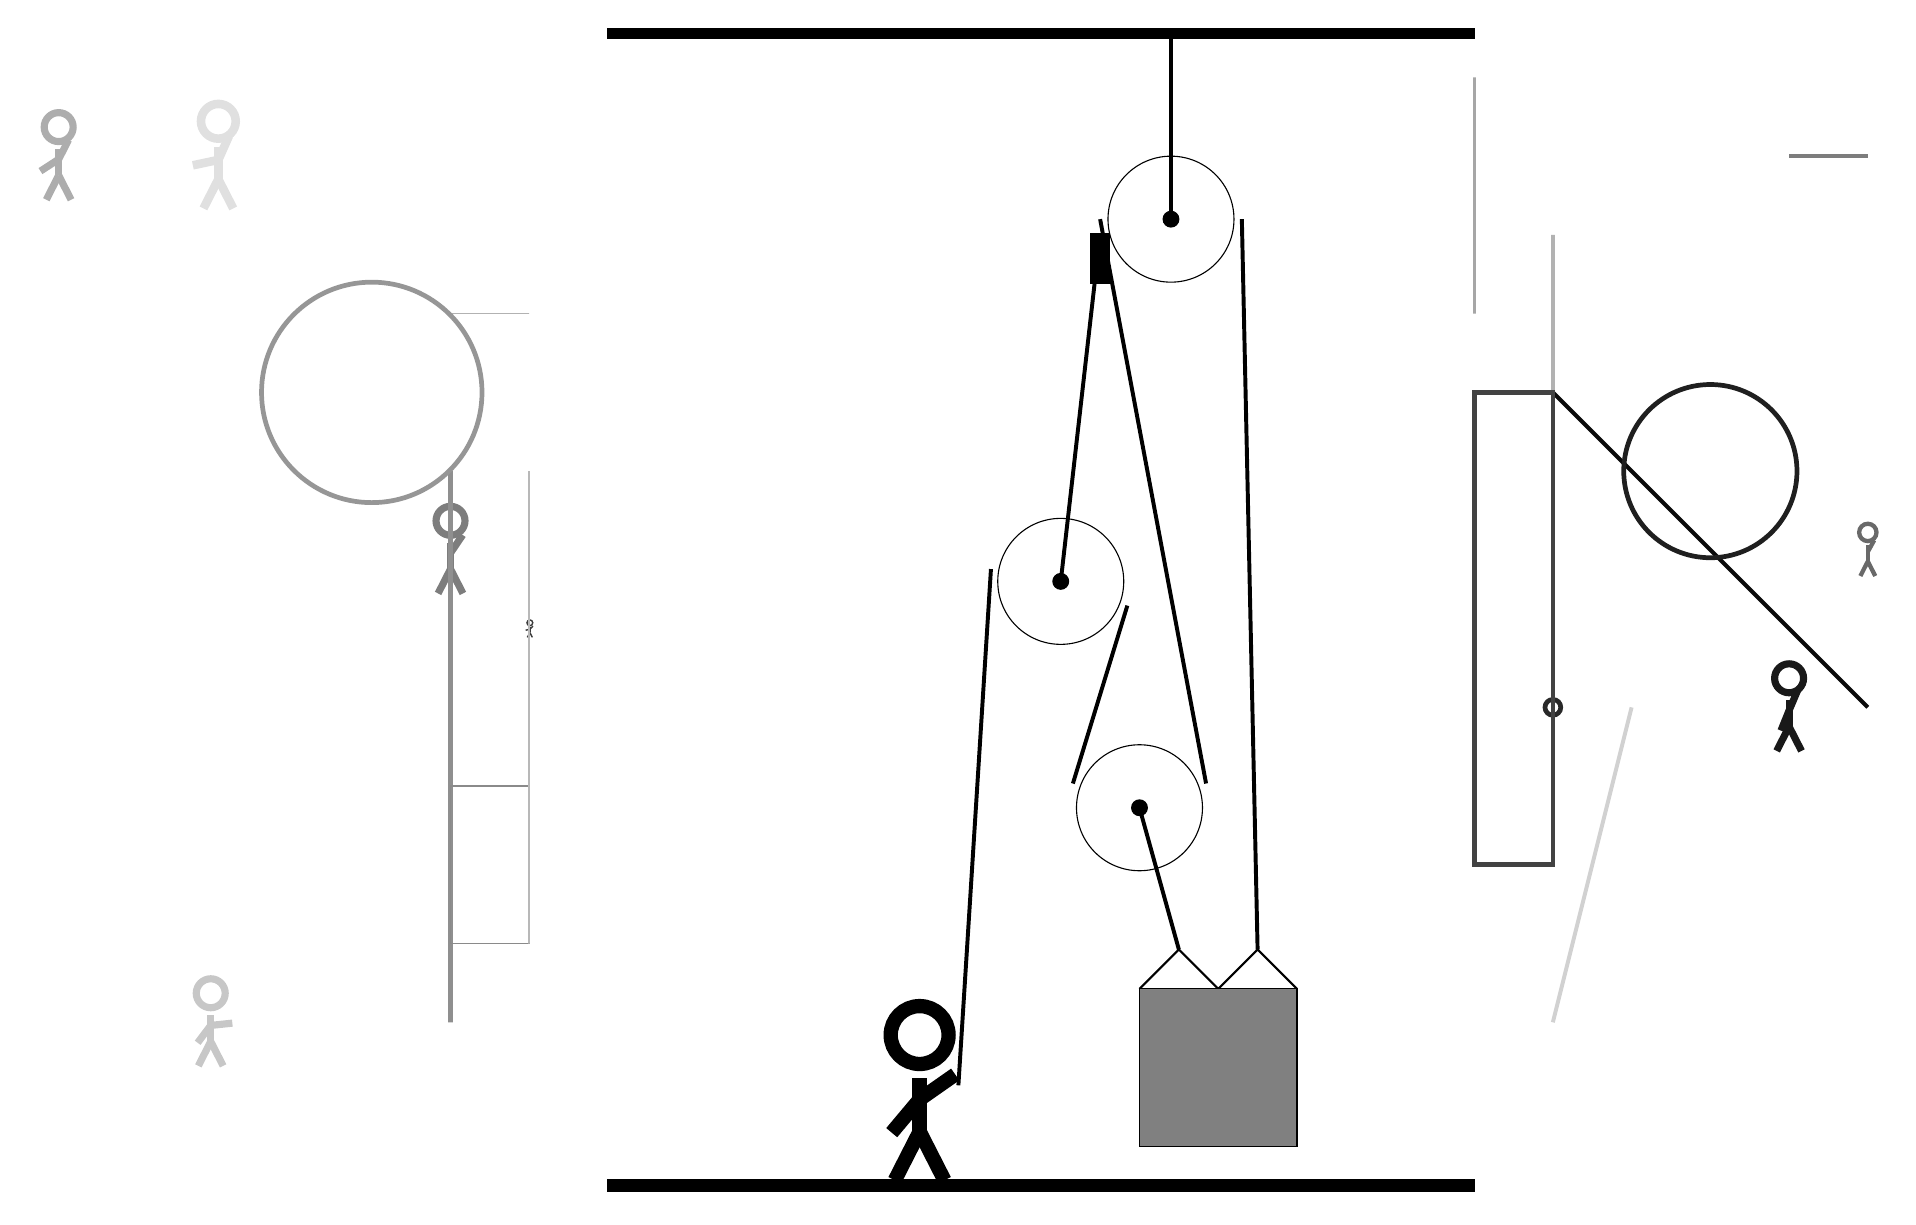
\begin{tikzpicture}
			%%%%% START %%%%%
			
			\draw[fill=black] (-6, 11.5) rectangle (5, 11.625);
			
			\draw (-0.25, 4.6) circle (0.8);
			\draw[fill=black] (-0.25, 4.6) circle (0.1);
			
			\draw (0.75, 1.725) circle (0.8);
			\draw[fill=black] (0.75, 1.725) circle (0.1);
			
			\draw (1.15, 9.2) circle (0.8);
			\draw[fill=black] (1.15, 9.2) circle (0.1);
			\draw[very thick] (1.15, 9.2) -- (1.15, 11.5);
			
			\draw[line width=0.5mm, color=black!96](6, 7) -- (10, 3);
			
			\node[line width=0.6mm, color=black!51] at (-8, 5) {\Strichmaxerl[5][90][56]};
			\node[line width=0.5mm, color=black!32] at (-13, 10) {\Strichmaxerl[5][33][63]};
			\node[line width=0.7mm, color=black!22] at (-11, -1) {\Strichmaxerl[5][53][6]};
			\node[line width=0.3mm, color=black!12] at (-11, 10) {\Strichmaxerl[6][12][66]};
			
			\node[line width=0.2mm, color=black!90] at (9, 3) {\Strichmaxerl[5][68][67]};
			
			\draw[line width=0.2mm, color=black!30] (-7, 8) rectangle (-8, 8);
			\draw[line width=0.4mm, color=black!35] (5, 8) rectangle (5, 11);
			\draw[line width=0.7mm, color=black!44] (-8, -1) rectangle (-8, 6);
			
			\draw[line width=0.6mm, color=black!30] (6, 1) rectangle (6, 9);
			\draw [line width=0.6mm, color=black!84](6, 3) circle (0.1);
			\draw [line width=0.6mm, color=black!41](-9, 7) circle (1.4);
			\draw[line width=0.5mm, color=black!51](9, 10) -- (10, 10);
			
			\draw[line width=0.6mm, color=black!74] (5, 1) rectangle (6, 7);
			\draw[line width=0.2mm, color=black!46] (-7, 2) rectangle (-8, 0);
			\draw [line width=0.6mm, color=black!88](8, 6) circle (1.1);
			\node[line width=0.3mm, color=black!76] at (-7, 4) {\Strichmaxerl[1][13][46]};
			
			\draw[line width=0.5mm, color=black!18](6, -1) -- (7, 3);
			\draw[line width=0.3mm, color=black!28] (-7, 6) rectangle (-7, 0);
			
			\node[line width=0.6mm, color=black!59] at (10, 5) {\Strichmaxerl[3][90][61]};
			
			\draw[thick]  (0.75, -0.575) -- (1.25, -0.075) -- (1.75, -0.575) -- (2.25, -0.075) -- (2.75, -0.575);
			\draw[fill=black!50] (0.75, -0.575) rectangle (2.75, -2.575);
			
			\draw[line width=0.5mm] (-0.25, 4.6) -- (0.25, 9.0);
			\draw[line width=0.5mm, fill=black](0.15, 8.4) rectangle (0.35, 9.0);
			\draw[line width=0.5mm] (-1.55, -1.8) -- (-1.1363, 4.7562);
			\centerarc[line width=0.5mm](-0.25, 4.6)(-20:170:0.9);
			\draw[line width=0.5mm] (0.5957, 4.2922) -- (-0.0957, 2.0328);
			\centerarc[line width=0.5mm](0.75, 1.725)(160:380:0.9);
			\draw[line width=0.5mm] (1.5957, 2.0328) -- (0.25, 9.2);
			\draw[line width=0.5mm](0.75, 1.725) -- (1.25, -0.075);
			\centerarc[line width=0.5mm](1.15, 9.2)(0:180:0.9);
			\draw[line width=0.5mm] (2.05, 9.2) -- (2.25, -0.075);
			
			\node at (-2, -1.9) {\Strichmaxerl[10][50][35]};
			
			\draw[fill=black] (-6, -3) rectangle (5, -3.15);
			
			%%%%% END %%%%%
		\end{tikzpicture}
	\end{figure}	
\end{document}